\documentclass[10pt]{article}

\usepackage[utf8]{inputenc}
\usepackage{amsmath}
\usepackage{amsthm}
\usepackage{amssymb}
\usepackage{bbm}
\usepackage{booktabs}
\usepackage{color}
\usepackage{enumerate}
\usepackage{framed}
\usepackage[margin=1in]{geometry}
\usepackage[pdftex]{graphicx}
\usepackage{epstopdf}
\usepackage{listings}
\usepackage{longtable}
\usepackage{multicol}
\usepackage{natbib}
\usepackage{paralist}
\usepackage{pdfpages}
\usepackage{setspace}
\usepackage{subfigure}
\usepackage{verbatim}
\usepackage{xcolor}
\usepackage{graphicx} % graphics
\usepackage{epsfig} % eps graphics
\usepackage{hyperref} % urls
\usepackage{booktabs} % table styling
\usepackage{overpic}
\usepackage{fix-cm}
\usepackage{rotating}
\usepackage{transparent}
\usepackage{attrib}
\usepackage{tikz}
\usepackage{multirow}
\usetikzlibrary{arrows,automata,3d}
\usepackage{epstopdf}
\usepackage{epigraph}
\usepackage{sgame}
\usetikzlibrary{calc}

\tikzset{
% Two node styles for game trees: solid and hollow
solid node/.style={circle,draw,inner sep=1.5,fill=black},
hollow node/.style={circle,draw,inner sep=1.5}
}

\newcommand{\tabitem}{~~\llap{\textbullet}~~}

\newcommand{\g}{\ensuremath{G}}
\newcommand{\strat}{\ensuremath{s}}
\newcommand{\strati}[1]{\ensuremath{s_{#1}}}
\newcommand{\stratpro}{\ensuremath{\mathbf{s}}}
\newcommand{\stratproi}[1]{\ensuremath{\mathbf{s}_{#1}}}
\newcommand{\besti}[2]{\ensuremath{B_{#1}\left(#2\right)}}
\newcommand{\EE}[1]{\ensuremath{\operatorname{E}\left[#1\right]}}
\newcommand{\condEE}[2]{\ensuremath{\operatorname{E}\left[#1\Big|#2\right]}}
\newcommand{\condpr}[2]{\ensuremath{\operatorname{Pr}\left[#1\Big|#2\right]}}
\newcommand{\pr}[1]{\ensuremath{\operatorname{Pr}\left[#1\right]}}


\newcommand{\solution}[2][no]{                                  % Replace "show" with any other word to hide solutions.
    \ifthenelse{ \equal{#1}{show} }{ \textcolor{blue}{#2}}{}}    % THIS FUNCTION LETS YOU WRITE IN SOLUTIONS BUT HIDE THEM WHEN RENDERING

\graphicspath{ {./img/}}

\title{Problem \#4}
\author{Ignacio Lara - Game Theory, Spring 2022}
\date{Due: Tuesday, April 26 by 8:30 AM Pacific}

\begin{document}

\maketitle

%\begin{figure}[h]
%  \centering
%    \includegraphics[width=0.5\textwidth]{../Cartoons/duck_rabbit_god.jpg}
%\end{figure}

Note: This problem is loosely based on a paper I wrote in graduate school, and also ties into work on ethnic diversity and economic growth from James Fearon, Alberto Alesina, and others.

\section*{A Model of Cross-Cultural Interaction}

In this problem we will investigate the incentives to invest in a public good when cultural differences result in people from different groups getting different payoffs from the public good. Models like this have been used to explain why certain countries have domestic instability and may break into smaller, more ethnically homogeneous countries (for example, Yugoslavia in the 1990s, or the Catalan separationist movement in Spain). You will see some ``testable implications" of the game that could be examined with data.

Suppose that there are two groups who have different cultures A and B. Think of this as two communities who interact and live in the same area but have different languages or slightly different cultural background. We will be modeling group-level payoffs, so you can also think of representative agents for the two groups.

Consumption can be either a culturally-specific consumption good that cannot be shared with others (e.g. food, entertainment, or religion) or a public good made through the contributions of both individuals and consumption can be shared (e.g. investments in local police or schools or arts; or at the country level something abstract like patriotism or concrete like national defense). Each group has 10 units of labor they can split between public and private consumption. Their contribution to the public good is $x_i$. Given both contributions, each group's payoff is $10-x_i+2(x_A+x_B)$. In this (admittedly simple) model, the private consumption is $10-x_i$ and public good consumption is $(x_A+x_B)$. They are interchangeable, but groups get twice as much utility per unit of public good, compared to the private good (e.g. there are economies of scale).

\subsection*{Part a} How much does each group choose to contribute to the public good, and what is each group's payoff?
\\ \\
Let $X = x_A + x_B$ represent total public good consumption. For group $i$, this can be rewritten as $X=x_i + x_{-i}$, where $x_{-i}$ refers to the contributions to the public good of the other group. Their payoff function is then
\[
10 - x_i + 2x_i + 2x_{-i} = 10 + x_i + 2x_{-i}
\]

Since every additional unit of $x_i$ results in an increased payoff, each group would contribute all 10 units of labor to the public good, such that $x_A^* = x_B^* = 10$ and each group receives a payoff of $10 - 10 + 2(20) = 40$. 
\newpage

\subsection*{Part b} Now suppose the cultures are sufficiently different that there is some cultural friction. Suppose culture $B$ is the majority culture, so $A$ faces a ``translation" cost (literally or figuratively, e.g. $B$'s cultural norms don't quite ``fit" $A$). This means that $A$'s payoff is reduced by a factor $\gamma<1$. So $A$'s payoff function is now $10-x_A+2\gamma(x_A+x_B)$. $B$'s payoff function is the same as before.

For what values of $\gamma$ will $A$ refuse to contribute to the public good? For those values of $\gamma$, how much will $B$ contribute, and what will be each group's utility?
\\ \\
Expand Group A's payoff function: $10 - x_A + 2\gamma x_A + 2\gamma x_B = 10 + (2\gamma - 1)x_A + 2\gamma x_B$. Group A would stop contributing to the public good once the additional contribution decreases their payoff. Since the marginal contribution of $x_A$ to A's payoff is linear (each unit of $x_A$ contributes $2\gamma - 1$ to A's payoff), A will not contribute to the public good if $2\gamma - 1 < 0$, i.e. $x_A^* = 0 \; \forall \: \gamma < 0.5$.
\\ \\
Assuming perfect information (i.e. B knows $\gamma$, and that $\gamma < 0.5$ results in $x_A^* = 0$), does that change B's optimum contribution to the public good?
\[
10 - x_B + 2(x_A + x_B) = 10 + x_B + 2x_A
\]
Even if $x_A = 0$, B still gets a linear marginal increase from $x_B$, so $x_B^* = 10$. This makes sense, because B's payoff is completely unaffected by $\gamma$, and the relative preference for \emph{B's own contribution} to the public vs. private good essentially makes the other group's contributions to the public good irrelevant.

Given $\gamma < 0.5 \Longrightarrow x_A^*=0, \: x_B^* = 10$, each group's payoff is:
\[
\begin{aligned}
	V_A^* &= 10 - 0 + 2\gamma(0 + 10) = 10 + 20\gamma \Longrightarrow V_A^* < 20\\
	V_B^* &= 10 - 10 + 2(0 + 10) = 20
\end{aligned}
\]
Each group's utility would be captured by their utility functions evaluated at these payoffs, $U_i(V_i^*)$.


\newpage

\subsection*{Part c} If group $A$ broke away and formed their own ``country," they could create their own public good, where the translation cost $\gamma$ is not an issue. Since group $B$ is no longer contributing, group $A$'s payoff function would then be $10-x+2x$, or $10+x$. For what values of $\gamma$ would group $A$ choose to leave, given what they would otherwise get in part b?
\\ \\
In part (b), Group A's payoffs as a function of $\gamma$ are
\[
\begin{cases}
	10 + 20\gamma, & \gamma < 0.5 \Longrightarrow (x_A^* = 0, \; x_B^*=10)\\
	40\gamma, & 0.5 \leq \gamma \leq 1 \Longrightarrow (x_A^* = x_B^* = 10)
\end{cases}
\]
(Technically, if $\gamma$ is exactly 0.5, A is indifferent between any $x_A \in \left[0, 10\right]$.) 
\\ \\
The question is for which values of $\gamma$ is A better off separating and receiving $10 + x$? If we assume that A still has only 10 units of labor, then A's maximum payoff if they separate is $10 + 10 = 20$. This is also the amount they would choose to produce (since $x$ still contributes linearly to their payoff). 

So we know that A is at least as well off without separating if $0.5 \leq \gamma \leq 1 \Longrightarrow 40\gamma \geq 20$; we can focus on the case where $\gamma < 0.5$. To start, find the value of $\gamma$ that would make A indifferent between separating and staying:
\[
\begin{aligned}
	10 + 20\gamma &\overset{?}{=} 20 \\
	20\gamma &\overset{?}{=} 10 \\
	\gamma &= 0.5
\end{aligned}
\]
A is strictly better off separating for any $\gamma < 0.5$. They might also choose to leave if $\gamma = 0.5$.


\newpage

\subsection*{Part d} Now let's expand so that we consider different-sized groups. Let there be $N$ people from culture $B$ and one person from $A$. (You can also think of this as the relative size of the cultures, i.e. culture $B$ is $N$ times as large as culture $A$.) Each person can contribute up to 10 to the public good. Let the contributions from culture $B$ be labeled $x_j$ for $j=1,\ldots,N$ and the person from $A$ still has contribution $x_A$. Then person $i$ from culture $B$ has payoff function $10-x_i+2\left(x_A+\sum_{j=1}^{N}x_j\right)$. The one person from $A$ has payoff function $10-x_A+2\gamma\left(x_A+\sum_{j=1}^{N}x_j\right)$.

For what values of $\gamma$, as a function of $N$, would group $A$ choose to leave and form their own country?
\\ \\
Intuitively, I would think the more disparate the two groups (i.e. with increasing $N$), the higher the translation cost would have to be to make separating more preferable for A than remaining (i.e. the critical $\gamma$ would be lower), because by separating, A is forgoing a larger total contribution to the public good.
\\ \\
A's payoff function is $10 + (2\gamma - 1)x_A + 2\gamma x_B$, where $x_B = \sum_{j=1}^N x_j$. So like before, A will not contribute anything to the public good if $\gamma < 0.5$. How can we tell what B will collectively contribute? Assuming a homogeneous population, we can just find the contribution for one individual $x_i$, then represent $x_B = Nx_i$. $i$'s payoff function is:
\[
10 - x_i + 2(x_A + \sum_{j=1}^{N} x_j) = 10 - x_i + 2x_A + 2x_B
\]

Like before, it does not depend on $\gamma$. But it does depend on everyone else in B, \emph{including} $i$'s contribution again! That is, the payoff for $i$ can be expanded to separate out $i$'s contribution to B's public good consumption:
\[
10 - x_i + 2(x_A + x_i + \sum_{j \neq i} x_j) = 10 - x_i + 2(x_A + x_i + (N-1)x_i)
\]

Note the last step in the RHS above relies on the homogeneous population assumption. That is, if everyone in B has the same $x_j$, then the contribution of B, minus one individual, is the sum of $(N-1)$ contributions, each of which are equal to the contribution of the individual ($x_B = x_i + (N-1)x_j, \quad x_i = x_j$). This simplifies $i$'s payoff function quite a bit:
\[
\begin{aligned}
10 - x_i + 2(x_A + x_i + (N-1)x_i) &= 10 - x_i + 2x_A + 2Nx_i \\
&= 10 + 2x_A + (2N-1)x_i
\end{aligned}
\]

Note that $x_i$ contributes linearly to $i$'s payoff, and it is a positive contribution only if $2N - 1 > 0 \Longrightarrow N > 0.5$. Thus, $i$ will contribute their maximum of 10 if $N > 0.5$, and contribute 0 if $N < 0.5$. This in turn means:
\[
x_B = \begin{cases}
	10N, & N > 0.5 \\
	0, & N < 0.5
\end{cases}
\]
(Again, if $N$ is exactly 0.5, $i$ is indifferent between any $x_i \in \left[0, 10\right]$, so $x_B \in \left[0, 10N\right]$.)
\\ \\
Return to A's payoff. If $N < 0.5$, B's contributions $x_B^* = 0$, so A's payoff is affected only by $\gamma$'s impact on $x_A$.
Like we said earlier, A does not contribute anything to the public good if $(2\gamma - 1) < 0 \Longrightarrow \gamma < 0.5$. Otherwise, $x_A$ contributes linearly to A's payoff, so $x_A^* = 10$. So, with zero contribution from B to the public good:
\[
V_A^* = \begin{cases}
	10 = 10 + 0 + 0, & \gamma < 0.5 \\
	20\gamma = 10 + 20\gamma - 10 + 0, & 0.5 \leq \gamma \leq 1
\end{cases}
\]
\\ \\
Now, if $N > 0.5 \Longrightarrow x_B^* = 10N$, so A's payoffs are:
\[
V_A^* = \begin{cases}
	10 + 20N\gamma, & \gamma < 0.5 \\
	20\gamma(N+1) = 20\gamma + 20N\gamma, & 0.5 \leq \gamma \leq 1
\end{cases}
\]
\\ \\
Almost home! The last step is to remember that A's payoff function becomes $10 + x$ if A separates, meaning their payoff $V_A^* = 20$. So, without separating, when is $V_A^* < 20$?
\\ \\
If $N < 0.5$:
\begin{itemize}
	\item $V_A^* = 10, \gamma < 0.5$ \textbf{Separate!}
	\item $V_A^* = 20\gamma, \gamma > 0.5 \therefore V_A^* < 20 \implies \gamma < 1$ \textbf{Separate!}
\end{itemize}
So A is better off alone regardless of any $\gamma < 1$ if $N < 0.5$.
\\ \\
If $N > 0.5$:
\begin{itemize}
	\item $V_A^* = 10 + 20N\gamma, \gamma < 0.5$
	\subitem $\therefore V_A^* < 20 \implies 20N\gamma < 10 \implies \gamma < \frac{1}{2N}$ 
	\subitem \textbf{Separate if $\gamma < \frac{1}{2N} \ \text{and} \ \gamma < 0.5$}
	\item $V_A^* = 20\gamma(N+1), 0.5 \leq \gamma \leq 1$
	\subitem $\therefore V_A^* < 20 \implies \gamma(N+1) < 1 \implies \gamma < \frac{1}{N+1}$ 
	\subitem \textbf{Separate if $\gamma < \frac{1}{N+1} \ \text{and} \ 0.5 \leq  \gamma \leq 1$}
\end{itemize}

Graphically (the shaded region is where A is better off separating):

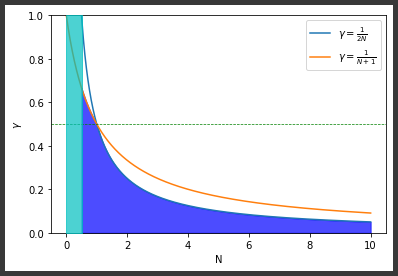
\includegraphics{culture_separate}
\newpage

\subsection*{Part e} Based on the answers above, which would we expect to be more stable: countries composed of many small but similar cultural subgroups, or countries with a few large but very different subgroups? Note that this is a testable implication: you could examine data on civil wars and ethnic composition to determine if our model appears supported by history.

Note: Cultural economists do take data to models like this, measuring ethnic fractionalization -- that is, the overall degree of heterogeneity in a country's population (Most often these measures are similar to the Herfindahl index of industry concentration, if you have seen that in an industrial organization context.) If you are interested in these papers, look up the work of James Fearon, Alberto Alesina, Enrico Spolaore, Jose Montalvo, and others. 

\end{document}
